\documentclass[a4paper,12pt,twoside]{memoir}

% Castellano
\usepackage[spanish,es-tabla]{babel}
\selectlanguage{spanish}
\usepackage[utf8]{inputenc}
\usepackage[T1]{fontenc}
\usepackage{lmodern} % scalable font
\usepackage{microtype}
\usepackage{placeins}

\RequirePackage{booktabs}
\RequirePackage[table]{xcolor}
\RequirePackage{xtab}
\RequirePackage{multirow}

% Links
\PassOptionsToPackage{hyphens}{url}\usepackage[colorlinks]{hyperref}
\hypersetup{
	allcolors = {red}
}

% Ecuaciones
\usepackage{amsmath}

% Rutas de fichero / paquete
\newcommand{\ruta}[1]{{\sffamily #1}}

% Párrafos
\nonzeroparskip

% Huérfanas y viudas
\widowpenalty100000
\clubpenalty100000

% Evitar solapes en el header
\nouppercaseheads

% Imagenes
\usepackage{graphicx}
\newcommand{\imagen}[2]{
	\begin{figure}[!h]
		\centering
		\includegraphics[width=0.9\textwidth]{#1}
		\caption{#2}\label{fig:#1}
	\end{figure}
	\FloatBarrier
}

\newcommand{\imagenflotante}[2]{
	\begin{figure}%[!h]
		\centering
		\includegraphics[width=0.9\textwidth]{#1}
		\caption{#2}\label{fig:#1}
	\end{figure}
}



% El comando \figura nos permite insertar figuras comodamente, y utilizando
% siempre el mismo formato. Los parametros son:
% 1 -> Porcentaje del ancho de página que ocupará la figura (de 0 a 1)
% 2 --> Fichero de la imagen
% 3 --> Texto a pie de imagen
% 4 --> Etiqueta (label) para referencias
% 5 --> Opciones que queramos pasarle al \includegraphics
% 6 --> Opciones de posicionamiento a pasarle a \begin{figure}
\newcommand{\figuraConPosicion}[6]{%
  \setlength{\anchoFloat}{#1\textwidth}%
  \addtolength{\anchoFloat}{-4\fboxsep}%
  \setlength{\anchoFigura}{\anchoFloat}%
  \begin{figure}[#6]
    \begin{center}%
      \Ovalbox{%
        \begin{minipage}{\anchoFloat}%
          \begin{center}%
            \includegraphics[width=\anchoFigura,#5]{#2}%
            \caption{#3}%
            \label{#4}%
          \end{center}%
        \end{minipage}
      }%
    \end{center}%
  \end{figure}%
}

%
% Comando para incluir imágenes en formato apaisado (sin marco).
\newcommand{\figuraApaisadaSinMarco}[5]{%
  \begin{figure}%
    \begin{center}%
    \includegraphics[angle=90,height=#1\textheight,#5]{#2}%
    \caption{#3}%
    \label{#4}%
    \end{center}%
  \end{figure}%
}
% Para las tablas
\newcommand{\otoprule}{\midrule [\heavyrulewidth]}
%
% Nuevo comando para tablas pequeñas (menos de una página).
\newcommand{\tablaSmall}[5]{%
 \begin{table}
  \begin{center}
   \rowcolors {2}{gray!35}{}
   \begin{tabular}{#2}
    \toprule
    #4
    \otoprule
    #5
    \bottomrule
   \end{tabular}
   \caption{#1}
   \label{tabla:#3}
  \end{center}
 \end{table}
}

%
%Para el float H de tablaSmallSinColores
\usepackage{float}

%
% Nuevo comando para tablas pequeñas (menos de una página).
\newcommand{\tablaSmallSinColores}[5]{%
 \begin{table}[H]
  \begin{center}
   \begin{tabular}{#2}
    \toprule
    #4
    \otoprule
    #5
    \bottomrule
   \end{tabular}
   \caption{#1}
   \label{tabla:#3}
  \end{center}
 \end{table}
}

\newcommand{\tablaApaisadaSmall}[5]{%
\begin{landscape}
  \begin{table}
   \begin{center}
    \rowcolors {2}{gray!35}{}
    \begin{tabular}{#2}
     \toprule
     #4
     \otoprule
     #5
     \bottomrule
    \end{tabular}
    \caption{#1}
    \label{tabla:#3}
   \end{center}
  \end{table}
\end{landscape}
}

%
% Nuevo comando para tablas grandes con cabecera y filas alternas coloreadas en gris.
\newcommand{\tabla}[6]{%
  \begin{center}
    \tablefirsthead{
      \toprule
      #5
      \otoprule
    }
    \tablehead{
      \multicolumn{#3}{l}{\small\sl continúa desde la página anterior}\\
      \toprule
      #5
      \otoprule
    }
    \tabletail{
      \hline
      \multicolumn{#3}{r}{\small\sl continúa en la página siguiente}\\
    }
    \tablelasttail{
      \hline
    }
    \bottomcaption{#1}
    \rowcolors {2}{gray!35}{}
    \begin{xtabular}{#2}
      #6
      \bottomrule
    \end{xtabular}
    \label{tabla:#4}
  \end{center}
}

%
% Nuevo comando para tablas grandes con cabecera.
\newcommand{\tablaSinColores}[6]{%
  \begin{center}
    \tablefirsthead{
      \toprule
      #5
      \otoprule
    }
    \tablehead{
      \multicolumn{#3}{l}{\small\sl continúa desde la página anterior}\\
      \toprule
      #5
      \otoprule
    }
    \tabletail{
      \hline
      \multicolumn{#3}{r}{\small\sl continúa en la página siguiente}\\
    }
    \tablelasttail{
      \hline
    }
    \bottomcaption{#1}
    \begin{xtabular}{#2}
      #6
      \bottomrule
    \end{xtabular}
    \label{tabla:#4}
  \end{center}
}

%
% Nuevo comando para tablas grandes sin cabecera.
\newcommand{\tablaSinCabecera}[5]{%
  \begin{center}
    \tablefirsthead{
      \toprule
    }
    \tablehead{
      \multicolumn{#3}{l}{\small\sl continúa desde la página anterior}\\
      \hline
    }
    \tabletail{
      \hline
      \multicolumn{#3}{r}{\small\sl continúa en la página siguiente}\\
    }
    \tablelasttail{
      \hline
    }
    \bottomcaption{#1}
  \begin{xtabular}{#2}
    #5
   \bottomrule
  \end{xtabular}
  \label{tabla:#4}
  \end{center}
}



\definecolor{cgoLight}{HTML}{EEEEEE}
\definecolor{cgoExtralight}{HTML}{FFFFFF}

%
% Nuevo comando para tablas grandes sin cabecera.
\newcommand{\tablaSinCabeceraConBandas}[5]{%
  \begin{center}
    \tablefirsthead{
      \toprule
    }
    \tablehead{
      \multicolumn{#3}{l}{\small\sl continúa desde la página anterior}\\
      \hline
    }
    \tabletail{
      \hline
      \multicolumn{#3}{r}{\small\sl continúa en la página siguiente}\\
    }
    \tablelasttail{
      \hline
    }
    \bottomcaption{#1}
    \rowcolors[]{1}{cgoExtralight}{cgoLight}

  \begin{xtabular}{#2}
    #5
   \bottomrule
  \end{xtabular}
  \label{tabla:#4}
  \end{center}
}




\graphicspath{ {./img/} }

% Capítulos
\chapterstyle{bianchi}
\newcommand{\capitulo}[2]{
	\setcounter{chapter}{#1}
	\setcounter{section}{0}
	\setcounter{figure}{0}
	\setcounter{table}{0}
	\chapter*{#2}
	\addcontentsline{toc}{chapter}{#2}
	\markboth{#2}{#2}
}

% Apéndices
\renewcommand{\appendixname}{Apéndice}
\renewcommand*\cftappendixname{\appendixname}

\newcommand{\apendice}[1]{
	%\renewcommand{\thechapter}{A}
	\chapter{#1}
}

\renewcommand*\cftappendixname{\appendixname\ }

% Formato de portada
\makeatletter
\usepackage{xcolor}
\newcommand{\tutor}[1]{\def\@tutor{#1}}
\newcommand{\course}[1]{\def\@course{#1}}
\definecolor{cpardoBox}{HTML}{E6E6FF}
\def\maketitle{
  \null
  \thispagestyle{empty}
  % Cabecera ----------------
\noindent
\includegraphics[width=\textwidth]{cabecera}\vspace{1cm}%
  \vfill
  % Título proyecto y escudo informática ----------------
  \colorbox{cpardoBox}{%
    \begin{minipage}{.8\textwidth}
      \vspace{.5cm}\Large
      \begin{center}
      \textbf{TFG del Grado en Ingeniería Informática}\vspace{.6cm}\\
      \textbf{\LARGE\@title{}}
      \end{center}
      \vspace{.2cm}
    \end{minipage}

  }%
  \hfill\begin{minipage}{.20\textwidth}
    
\includegraphics[width=\textwidth]{escudoInfor}
  \end{minipage}
  \vfill
  % Datos de alumno, curso y tutores ------------------
  \begin{center}%
  {%
    \noindent\LARGE
    Presentado por \@author{}\\ 
    en Universidad de Burgos --- \@date{}\\
    Tutor: \@tutor{}\\
  }%
  \end{center}%
  \null
  \cleardoublepage
  }
\makeatother


% Datos de portada
\title{título del TFG \\Documentación Técnica}
\author{Víctor De Marco Velasco}
\tutor{Carlos Cambra Baseca}
\date{\today}

\begin{document}

\maketitle



\cleardoublepage



%%%%%%%%%%%%%%%%%%%%%%%%%%%%%%%%%%%%%%%%%%%%%%%%%%%%%%%%%%%%%%%%%%%%%%%%%%%%%%%%%%%%%%%%



\frontmatter


\clearpage

% Indices
\tableofcontents

\clearpage

\listoffigures

\clearpage

\listoftables

\clearpage

\mainmatter

\appendix

\apendice{Plan de Proyecto Software}

\section{Introducción}
En este apartado se explica la planificación temporal seguida durante el proyecto y el estudio de cuán viable es tanto en el ámbito económico como legal.
	
\section{Planificación temporal}
La planificación temporal del proyecto se ha llevado a cabo utilizando Sprints haciendo referencia a la metodología Scrum. La duración, el objetivo y cómo cumplir dicho objetivo en cada Sprint deben decidirse entre los integrantes que van a formar parte del proyecto antes de comenzar el Sprint.
Cuando llega la fecha límite acordada se comprueba si ha sido posible realizar todo lo planificado durante la reunión de creación del Sprint. Según lo que se haya logrado realizar se actualizan los objetivos y tareas del proyecto. Esto continúa hasta que se da por finalizado el proyecto.
\section{Estudio de viabilidad}
El estudio de viabilidad del proyecto se ha realizado desde el punto de vista económico y legal.
\subsection{Viabilidad económica}
Para poder determinar si un proyecto software es viable económicamente, se deben calcular los gastos que supondría realizar el proyecto y los beneficios que se podrían obtener del mismo. Una vez realizados estos cálculos se puede determinar si el proyecto es un proyecto viable desde el punto de vista económico.
\subsubsection{Costes Hardware}
Para realizar este proyecto se ha necesitado:
\begin{itemize}
    \item Ordenador portátil Asus: 900€
    \item Dragino LoRaWAN Gateway: 165€
    \item Merry IoT Motion Detection: 45€
\end{itemize}
Teniendo en cuenta la vida útil económica de estos dispositivos, el coste anual de cada uno sería:
\begin{itemize}
    \item Ordenador portátil Asus (4 años): 225€
    \item Dragino LoRaWAN Gateway (5 años): 33€
    \item Merry IoT Motion Detection (6 años): 7,5€
\end{itemize}
Aunque estos dispositivos seguramente podrían seguir usándose pasada la vida útil contemplada, debido a posibles mejoras técnicas y  nuevas tecnologías superiores a estos dispositivos convendría actualizarlos y prescindir de ellos. 
\subsubsection{Costes Software}
Para realizar este proyecto se ha necesitado:
\begin{itemize}
    \item Sistema operativo Windows 11: 145€
    \item Dominio web: 4,55€
\end{itemize}
Aclarar que la compra del dominio web se paga de forma anual y el sistema operativo se amortiza dependiendo del dispositivo en el que este instalado, por lo tanto dispone de 4 años de vida útil al estar en el ordenador portátil Asus.
\subsubsection{Coste de Desarrollo}
Considerando que el proyecto lo he desarrollado yo solo el único coste de desarrollo a tener en cuenta seria mi sueldo.
\begin{itemize}
    \item Sueldo anual: 6.240€
    \item Sueldo mensual: 520€
\end{itemize}
Este sueldo esta calculado suponiendo que se trabaja 40 horas mensuales.
\subsubsection{Costes Adicionales}
De momento no se ha necesitado añadir ningún coste adicional no planteado anteriormente.
\subsubsection{Coste Total}
Suponiendo que se llevara a cabo el proyecto durante un año vamos a calcular el coste del mismo:
\begin{table}[H]
\centering
\begin{tabular}{|l|c|c|p{5cm}|}
\hline
\textbf{Elemento} & \textbf{Coste Anual (€)} & \textbf{Comentario} \\
\hline
Hardware: Portatil Asus & 225  & Vida útil 4 años. \\
\hline
Hardware: Gateway Dragino & 33  & Vida útil 5 años. \\
\hline
Hardware: Sensor MerryIoT & 7,5  & Vida útil 6 años. \\
\hline
Software: Dominio web & 4,55 & Uso exclusivo para el proyecto. \\
\hline
Software: Windows 11 & 36,25  & Licencia del sistema operativo \\
\hline
Horas de desarrollo & 6240  & Sueldo aproximado \\
\hline
\textbf{TOTAL} & 6.546,3  & Coste total de un año de desarrollo \\
\hline
\end{tabular}
\caption{Resumen de costes estimados durante un año}
\label{tab:viabilidad-economica}
\end{table}
Una vez observados los cálculos pretender sacar rédito económico del proyecto parece no ser muy realista ya que es un proyecto que individualmente no tiene mucho interés comercial, seria mas como parte de un proyecto mucho mas grande. 

\subsection{Viabilidad legal}
Para poder determinar si un proyecto es viable legalmente se deben revisar las licencias utilizadas durante el proyecto y determinar si hay alguna barrera legal que impida el desarrollo y uso del proyecto.

\subsubsection{Marco legal}

El proyecto se desarrolla en España, por lo que hay que cumplir con las siguientes normativas:

\begin{itemize}
    \item Reglamento (UE) 2016/679 del Parlamento Europeo y del Consejo, de 27 de abril de 2016, relativo a la protección de las personas físicas (RGPD).
    \item Ley Orgánica 3/2018, de 5 de diciembre, de Protección de Datos Personales y garantía de los derechos digitales (LOPDGDD).
    \item Ley de Propiedad Intelectual (Real Decreto Legislativo 1/1996, de 12 de abril).
    \item Licencias de uso de software libre y de terceros (MIT, GPL, etc.).
\end{itemize}

\subsubsection{Protección de datos personales}

El proyecto en ningún momento recoge datos personales de ningún tipo ya que los únicos datos procesados corresponden a lecturas del sensor IoT ubicado en mi domicilio.
Por tanto, no existe tratamiento de datos personales según el RGPD.

\subsubsection{Licencias y uso de software}

El proyecto utiliza las siguientes tecnologías software:

\begin{itemize}
    \item \textbf{Windows 11}: sistema operativo bajo licencia instalada en el equipo de desarrollo.
    \item \textbf{IntelliJ IDEA}: utilizado en su versión Community Edition, que se distribuye bajo licencia Apache 2.0.
    \item \textbf{Python y Flask}: ambos distribuidos bajo licencias permisivas (Python Software Foundation License y BSD, respectivamente).
    \item \textbf{Cloudflared Tunnel}: herramienta libre para crear túneles seguros, distribuida bajo licencia Apache 2.0.
    \item \textbf{The Things Network (TTN)}: plataforma en la nube gratuita para LoRaWAN, utilizada según sus condiciones de uso.
    \item \textbf{Dominio web}: contratado para uso exclusivo del proyecto durante un año.
\end{itemize}

Todos los recursos software utilizados permiten su uso académico sin restricción y se respetan las licencias correspondientes.

\subsubsection{Uso de hardware}

El hardware utilizado incluye un gateway LoRaWAN Dragino y un sensor MerryIoT de detección de movimiento y condiciones ambientales. Ambos dispositivos se han instalado en mi domicilio por lo tanto no se ha realizado ninguna instalación en un espacio público ni se requiere certificación adicional, ya que ambos operan en bandas ISM de uso libre y conforme a normativa europea.

\subsubsection{Conclusión}

En conclusión  el proyecto es legalmente viable, no vulnera la normativa de protección de datos ni derechos de terceros, y respeta las condiciones de uso de todo el software y hardware utilizado.




\apendice{Especificación de Requisitos}

\section{Introducción}

En este apartado se describen los objetivos generales del proyecto, los requisitos tanto funcionales como no funcionales y los distintos casos de uso del software.

% Caso de Uso 1 -> Consultar Experimentos.
%\begin{table}[p]
%	\centering
%	\begin{tabularx}{\linewidth}{ p{0.21\columnwidth} p{0.71\columnwidth} }
%		\toprule
%		\textbf{CU-1}    & \textbf{Ejemplo de caso de uso}\\
%		\toprule
%		\textbf{Versión}              & 1.0    \\
%		\textbf{Autor}                & Alumno \\
%		\textbf{Requisitos asociados} & RF-xx, RF-xx \\
%		\textbf{Descripción}          & La descripción del CU \\
%		\textbf{Precondición}         & Precondiciones (podría haber más de una) \\
%		\textbf{Acciones}             &
%		\begin{enumerate}
%			\def\labelenumi{\arabic{enumi}.}
%			\tightlist
%			\item Pasos del CU
%			\item Pasos del CU (añadir tantos como sean necesarios)
%		\end{enumerate}\\
%		\textbf{Postcondición}        & Postcondiciones (podría haber más de una) \\
%		\textbf{Excepciones}          & Excepciones \\
%		\textbf{Importancia}          & Alta o Media o Baja... \\
%		\bottomrule
%	\end{tabularx}
%	\caption{CU-1 Nombre del caso de uso.}
%\end{table}
%
\section{Objetivos generales}
\begin{enumerate}

    \item Obtener datos ambientales (temperatura, humedad y detección de movimiento) desde sensores LoRaWAN instalados en el entorno doméstico.
    \item Transmitir dichos datos obtenidos a través de un gateway Dragino hacia la red The Things Network (TTN).
     \item Recibir los datos enviados por TTN mediante un webhook HTTP a través de una aplicación web desarrollada en Python (Flask) y alamacenar los datos recibidos en un fichero CSV estructurado para su posterior análisis.
    \item Procesar y visualizar los datos mediante una aplicación web desarrollada con Python y Flask.
    

\end{enumerate}
\section{Catálogo de requisitos}
Una vez claros los objetivos generales del proyecto podemos definir los requisitos del mismo:
\subsubsection{Requisitos funcionales}

\begin{itemize}
    \item \textbf{RF1-Recopilación de datos}: El sistema debe recoger datos de temperatura, humedad y detección de movimiento desde sensores LoRaWAN.
    \item \textbf{RF2-Reconducir la información}: 
    \begin{itemize}
    \item \textbf{RF2.1}:El gateway Dragino debe reenviar los datos recogidos hacia la red The Things Network (TTN).
    \item \textbf{RF2.2}: Los datos recogidos deben ser transformados gracias a un payload formatter configurado.
    \item \textbf{RF2.3}: La aplicación Flask debe recibir peticiones POST desde TTN mediante un webhook HTTP.
    \end{itemize}
    \item \textbf{RF3-Almacenamiento de datos}:
    \begin{itemize}
    \item \textbf{RF3.1}: La aplicación web encargada de recibir los datos verifica la existencia de un fichero csv con el formato correcto para almacenar nuestros datos.
    \item \textbf{RF3.2}: La aplicación web comprueba que los datos que recibe son procesables y notifica al usuario si hay algún error o si todo va según lo previsto. 
    \item \textbf{RF3.3}: La aplicación web añade el paquete recibido en la ultima fila del fichero csv.
    \end{itemize}
    \item \textbf{RF4-Visualización web}:
    \begin{itemize}
    \item \textbf{RF4.1}: La aplicación web realiza una diferenciación entre los datos recopilados reales y los datos infectados.
    \item \textbf{RF4.2}: La aplicación web muestra las gráficas correspondientes a los datos reales recopilados.
    \item \textbf{RF4.3}: La aplicación web permite al usuario navegar entre las distintas opciones de datos (reales, infectados, todos).
    \end{itemize}
\end{itemize}
\subsubsection{Requisitos no funcionales}

\begin{itemize}
    \item \textbf{RNF1-Rendimiento}: El sistema debe estar disponible siempre que el usuario lo requiera y tener un bajo tiempo de respuesta.
    \item \textbf{RNF2-Seguridad}: El túnel expuesto mediante Cloudflare debe permitir comunicación segura entre TTN y el servidor local, sin suponer un problema de seguridad para los usuarios.
    \item \textbf{RNF3-Usabilidad}: El fichero CSV debe tener una estructura homogénea y legible para permitir su análisis posterior y su fácil utilización si el usuario necesitara manipularlo.
    \item \textbf{RNF4-Compatibilidad}: El sistema debe funcionar correctamente desde los distintos navegadores web mas populares.
    \item \textbf{RNF5-Mantenimiento}: El programa debe tener una estructura limpia y clara para facilitar el mantenimiento y añadir mas funciones a futuro.
\end{itemize}
\section{Especificación de requisitos}
En este apartado se especifican los distintos casos de uso de nuestro proyecto:

\begin{table}[p]
	\centering
	\begin{tabularx}{\linewidth}{ p{0.21\columnwidth} p{0.71\columnwidth} }
		\toprule
		\textbf{CU-1}    & Recopilar datos desde sensores LoRaWAN \\
		\toprule
		\textbf{Versión}              & 1.0 \\
		\textbf{Autor}                & Víctor De Marco Velasco \\
		\textbf{Requisitos asociados} & RF1 \\
		\textbf{Descripción}          & El sistema recibe datos ambientales (temperatura, humedad y detección de movimiento) a través de sensores LoRaWAN instalados en un entorno doméstico. \\
		\textbf{Precondición}         & El sensor debe estar encendido y correctamente enlazado con el gateway LoRaWAN. \\
		\textbf{Acciones}             &
		\begin{enumerate}
			\item El sensor realiza una medición periódica.
			\item El sensor transmite los datos al gateway Dragino.
		\end{enumerate}\\
		\textbf{Postcondición}        & El gateway recibe el paquete con los datos del sensor. \\
		\textbf{Excepciones}          & El sensor no transmite por fallo de batería o conectividad. \\
		\textbf{Importancia}          & Alta \\
		\bottomrule
	\end{tabularx}
	\caption{CU-1 Recopilar datos desde sensores LoRaWAN}
\end{table}
\begin{table}[p]
	\centering
	\begin{tabularx}{\linewidth}{ p{0.21\columnwidth} p{0.71\columnwidth} }
		\toprule
		\textbf{CU-2}    & Reenviar y transformar datos mediante TTN \\
		\toprule
		\textbf{Versión}              & 1.0 \\
		\textbf{Autor}                & Víctor De Marco Velasco \\
		\textbf{Requisitos asociados} & RF2.1, RF2.2, RF2.3 \\
		\textbf{Descripción}          & El gateway envía los datos a la red TTN, donde son decodificados mediante un payload formatter y redirigidos a la aplicación Flask mediante webhook. \\
		\textbf{Precondición}         & El gateway debe estar conectado a Internet y configurado correctamente en TTN. \\
		\textbf{Acciones}             &
		\begin{enumerate}
			\item El gateway Dragino reenvía los datos al servidor TTN.
			\item TTN aplica el payload formatter para decodificar los datos.
			\item TTN envía los datos a la aplicación Flask a través del webhook HTTP.
		\end{enumerate}\\
		\textbf{Postcondición}        & La aplicación Flask recibe un POST con los datos decodificados. \\
		\textbf{Excepciones}          & Fallo de red, error en el payload formatter o caída del túnel. \\
		\textbf{Importancia}          & Alta \\
		\bottomrule
	\end{tabularx}
	\caption{CU-2 Reenviar y transformar datos mediante TTN}
\end{table}
\begin{table}[p]
	\centering
	\begin{tabularx}{\linewidth}{ p{0.21\columnwidth} p{0.71\columnwidth} }
		\toprule
		\textbf{CU-3}    & Almacenar datos en archivo CSV \\
		\toprule
		\textbf{Versión}              & 1.0 \\
		\textbf{Autor}                & Víctor De Marco Velasco \\
		\textbf{Requisitos asociados} & RF3.1, RF3.2, RF3.3 \\
		\textbf{Descripción}          & La aplicación Flask verifica el CSV de almacenamiento, comprueba los datos recibidos y los añade correctamente como nueva fila. \\
		\textbf{Precondición}         & El webhook ha entregado correctamente los datos. \\
		\textbf{Acciones}             &
		\begin{enumerate}
			\item La aplicación verifica si el archivo CSV existe y contiene las cabeceras.
			\item Valida que el contenido recibido sea procesable.
			\item Añade una nueva fila con los datos recibidos.
			\item Informa si ha habido un error o se ha completado la operación correctamente.
		\end{enumerate}\\
		\textbf{Postcondición}        & El CSV contiene una nueva fila de datos válidos. \\
		\textbf{Excepciones}          & Formato incorrecto del payload, error de escritura, archivo dañado. \\
		\textbf{Importancia}          & Alta \\
		\bottomrule
	\end{tabularx}
	\caption{CU-3 Almacenar datos en archivo CSV}
\end{table}
\begin{table}[p]
	\centering
	\begin{tabularx}{\linewidth}{ p{0.21\columnwidth} p{0.71\columnwidth} }
		\toprule
		\textbf{CU-4}    & Visualizar datos en la aplicación web \\
		\toprule
		\textbf{Versión}              & 1.0 \\
		\textbf{Autor}                & Víctor De Marco Velasco \\
		\textbf{Requisitos asociados} & RF4.1, RF4.2, RF4.3 \\
		\textbf{Descripción}          & El usuario puede acceder a una interfaz web para consultar los datos recogidos en formato visual y filtrarlos por tipo. \\
		\textbf{Precondición}         & El archivo CSV contiene datos válidos. \\
		\textbf{Acciones}             &
		\begin{enumerate}
			\item El usuario accede a la aplicación web.
			\item Selecciona el tipo de datos a visualizar (reales, infectados, todos).
			\item La aplicación carga los datos desde el CSV.
			\item Se muestran las gráficas o tablas correspondientes.
		\end{enumerate}\\
		\textbf{Postcondición}        & El usuario visualiza los datos filtrados correctamente. \\
		\textbf{Excepciones}          & El CSV está corrupto o no se puede leer, o hay error en los filtros. \\
		\textbf{Importancia}          & Media \\
		\bottomrule
	\end{tabularx}
	\caption{CU-4 Visualizar datos en la aplicación web}
\end{table}


\apendice{Especificación de diseño}

\section{Introducción}
En este apartado se documentan los datos , la arquitectura, el procedimiento y la guía de estilo del proyecto.
\section{Diseño de datos}

El almacenamiento de datos se realiza en un fichero CSV denominado \texttt{webhook\_dataset.csv}, generado y mantenido por la aplicación Flask. Cada fila del fichero representa un conjunto de datos recibidos de TTN.

Los campos de los datos recibidos son los siguientes:

\begin{itemize}
    \item \textbf{timestamp}: Fecha y hora de recepcion del mensaje.
    \item \textbf{occupied (boolean)}: Indica si se detectó movimiento en su campo de visión.
    \item \textbf{button\_pressed (boolean)}: Estado del botón del sensor.
    \item \textbf{tamper\_detected (boolean)}: Detección de presencia.
    \item \textbf{battery\_voltage (float)}: Voltaje actual de la batería (V).
    \item \textbf{temperature\_celsius (int)}: Temperatura medida (ºC).
    \item \textbf{humidity\_percent (int)}: Humedad relativa (\%).
    \item \textbf{time\_since\_last\_event\_min (int)}: Minutos desde el último evento.
    \item \textbf{event\_count (int)}: Contador de eventos.
\end{itemize}

Por último, la aplicación añade un campo más (estado) y le otorga el valor correspondiente al resultado obtenido en el análisis del paquete de datos recibido.

Todos los datos son almacenados en texto plano, separados por comas y con codificación UTF-8.

Además en este proyecto se ha utilizado una base de datos SQL encargada de almacenar y gestionar los credenciales de inicio de sesión de los diferentes usuarios que quieran usar la aplicación.

Por último, cada usuario puede almacenar diversos ficheros csv en su lista de ficheros csv personal. Todo fichero que se encuentre en esa lista podrá ser utilizado por el usuario. para aplicar las diversas funcionalidades de la aplicación. Los ficheros cargados en la aplicación para ser analizados también son guardados en esta lista tras el análisis. 

\section{Diseño arquitectónico}
En este apartado se van a mostrar las distintas estructuras utilizadas durante el desarrollo del proyecto.

\subsection{Modelo-Vista-Controlador (MVC)}

El patrón MVC es un patrón de diseño muy utilizado en aplicaciones web. Divide una aplicación en tres componentes principales:

\begin{itemize}
    \item Modelo: Gestiona los datos (modificar, almacenar\ldots).
    \item Vista: Se encarga de mostrar los datos al usuario. Es la parte visual de la aplicación (interfaz).
    \item Controlador: Intermediario entre la vista y el modelo. Recibe las peticiones del usuario, llama al modelo y selecciona la vista adecuada para la respuesta.
\end{itemize}

\subsubsection{Modelo}
En el proyecto el Modelo estaría representado por las funciones que leen, procesan y almacenan datos en esos archivos o los propios archivos csv donde se almacenan los datos.

\subsubsection{Vista}
En el proyecto la Vista estaría representada en las gráficas que la aplicación muestra al usuario tras aplicar un fichero csv o la visualización del contenido de un paquete antes de que el usuario decida enviarlo al dataset.

\subsubsection{Controlador}
En el proyecto, el Controlador estaría representado por los formularios que permiten al usuario introducir valores que serán utilizados por el programa para desempeñar distintas funciones o los botones con los que el usuario puede interactuar para llevar a cabo una acción.

\subsection{Frontend y Backend}

En el proyecto desarrollado se nota una clara diferenciación entre el frontend y el backend. La primera aplicación webhook\_flask esta centrada en el backend mientras que la segunda aplicación dashboard\_flask se centra en el frontend.

\subsubsection{Frontend}
dashboard\_flask es la aplicación encargada de todas las funcionalidades relacionadas con interactuar con el usuario y permitir al mismo disfrutar de la lógica detrás de las funciones del backend sin que este tenga que entender el funcionamiento de las mismas.

\subsubsection{Backend}
webhook\_flask en cambio es la aplicación más centrada en procesamiento de datos y comprobación de que el flujo de datos con la red LoRaWAN este funcionando correctamente, para permitir así al usuario disfrutar plenamente de las funciones que ofrece el proyecto.

Esta clara separación entre las dos aplicaciones facilita la organización y mantenimiento del proyecto, ademas de ayudar al desarrollo de nuevas funcionalidades en el futuro.


\subsection{Arquitectura del proyecto}
La arquitectura final del proyecto desarrollado es:

\imagen{arquitectura}{Arquitectura del proyecto}

Los rectángulos azules hacen referencia a la parte del proyecto más relacionada con una red LoRaWAN, es la parte que no he tenido que desarrollar, sino configurar para asegurar su correcto funcionamiento durante el desarrollo del proyecto.

Los rectángulos amarillos hacen referencia a las dos aplicaciones web que he desarrollado para lograr los objetivos del proyecto.

El rectángulo verde representa el archivo csv denominado webhook\_dataset, el archivo principal del proyecto y con el que ambas aplicaciones interactúan.

Por último se representa con un rectángulo blanco al usuario, el cual interactúa con el proyecto a través de la primera aplicación web.

\section{Diseño procedimental}
A continuación se muestran distintos diagramas referentes a distintas acciones que se llevan a cabo durante el proyecto.

La \autoref{fig:C2} representa el caso de recepción y almacenamiento de datos.

La \autoref{fig:C3} representa el caso de carga de archivos csv.

\begin{figure}
    \centering
    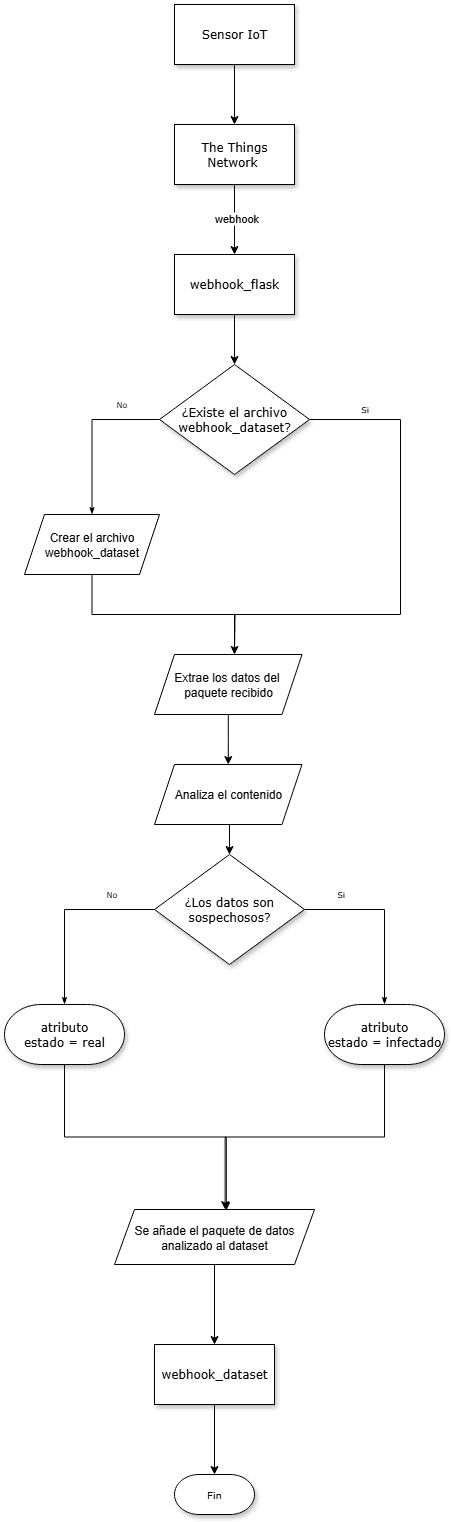
\includegraphics[width=0.5\textwidth]{recibir} 
    \caption{Diagrama de recepción y almacenamiento de datos.}
    \label{fig:C2}
\end{figure}


\begin{figure}
    \centering
    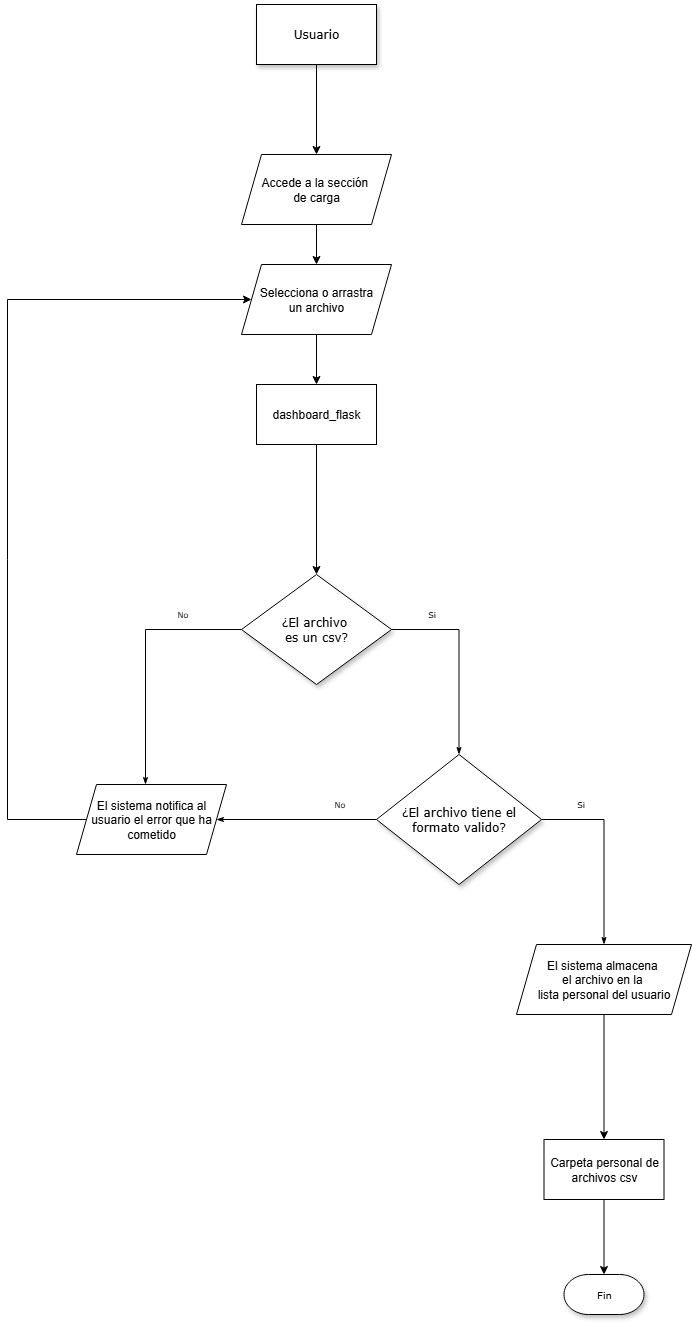
\includegraphics[width=0.8\textwidth]{cargar} 
    \caption{Diagrama de carga de archivos csv.}
    \label{fig:C3}
\end{figure}
\apendice{Documentación técnica de programación}

\section{Introducción}

\section{Estructura de directorios}

\section{Manual del programador}

\section{Compilación, instalación y ejecución del proyecto}

\section{Pruebas del sistema}

\apendice{Documentación de usuario}

\section{Introducción}

\section{Requisitos de usuarios}

\section{Instalación}

\section{Manual del usuario}



\apendice{Anexo de sostenibilización curricular}

\section{Introducción}
Este anexo incluirá una reflexión personal del alumnado sobre los aspectos de la sostenibilidad que se abordan en el trabajo.

La reflexión se ha realizado según las directrices estipuladas en el documento  sobre la introducción de la sostenibilidad de la CRUE \cite{Sos}.


\section{Competencias de sostenibilidad
adquiridas}

\begin{itemize}
    \item \textbf{Contextualización crítica del conocimiento (SOS1)}: En el trabajo he procurado analizar no solo el problema técnico planteado, sino también su relación con el entorno social y su posible repercusión ambiental. Esta visión me ha ayudado a comprender cómo una solución aparentemente eficiente puede no ser sostenible si no se considera su contexto.
    \item \textbf{Uso sostenible de recursos (SOS2)}: A lo largo del trabajo he sido consciente de la necesidad de aplicar criterios de eficiencia y reducción del consumo computacional en la fase de pruebas o despliegue, cuando ha sido posible.
    \item \textbf{Participación comunitaria (SOS3)}: Durante el desarrollo del proyecto he intentado tener en cuenta las necesidades de posibles usuarios y comunidades relacionadas con el tema tratado en el proyecto. La sostenibilidad también implica diseñar soluciones accesibles, inclusivas y que respondan a demandas reales.
    \item \textbf{Principios éticos (SOS4)}: He reflexionado sobre el impacto ético de las tecnologías tratadas, evitando decisiones que pudieran contribuir a la exclusión o la injusticia social. La sostenibilidad y equidad, ha sido un criterio clave en la toma de decisiones.
\end{itemize}



\section{Conclusiones}
EL desarrollo de este proyecto no solo ha aumentado mis conocimientos técnicos sobre diversos campos de la informática, sino que además he aprendido la importancia de tener en cuenta los principios de sostenibilidad aplicados a la informática a la hora de desarrollar un proyecto.  




\bibliographystyle{plain}
\bibliography{bibliografiaAnexos}

\end{document}
